\subsubsection{Equity Variance and Volatility Swap}
\label{pricing:eq_varianceswap}

Equity Variance and volatility swaps are priced using a replicating portfolio method \cite{Variance_Swaps_JP_Morgan}. A
variance swap can be theoretically replicated by a hedged portfolio of vanilla equity options on the same underlying
with a range of strikes. The price of the variance swap involves the cost of the replicating portfolio as per below. The
variance swap is then priced as

\begin{equation}\label{eq_varianceswap_payoff}
P(0,T) \cdot \omega \cdot N_{var} \cdot 10000 \cdot ( Var - K_{var}  )
\end{equation}

A volatility swap on the other hand is priced as

\begin{equation}
P(0,T) \cdot \omega \cdot N_{vol} \cdot 100 \cdot ( Vol - K_{vol} )
\end{equation}

where:

\begin{itemize}
\item $\omega \in \{-1,1\}$ is $1$ for a long and $-1$ for a short position
\item $K_{var} = K_{vol}^2$ is the variance strike which by definition is the square of the volatility strike $K_{vol}$
  given in the trade xml node ``Strike''
\item $N_{var}$ is the variance notional which by convention is given by
  $$N_{var} = \frac{N_{vol}}{2 \cdot 100 \cdot K_{vol}}$$
  Here the vega notional $N_{vol}$ is given in the trade xml node ``Notional''
\item $Var$ is the annualized realized variance of RIC:.SPX at the end date of the trade
\item $Vol = E( \sqrt{Var} )$ is the expected volatility
\item $P(0,T)$: the discount factor on the relevant OIS collateral curve for maturity time $T$
\end{itemize}

Accrued variance is handled by taking advantage of the additivity of the variance formula (after accounting for
time). The future variance can be replicated (see \cite{Variance_Swaps_JP_Morgan}, 4.5):

\begin{equation}\label{eq_varianceswap_replication}
\text{Variance} = \frac{2}{T} \left[ \int_0^F \frac{P(K)}{K^2} dK + \int_F^\infty \frac{C(K)}{K^2} dK \right]
\end{equation}

where $P(K)$, $C(K)$ are non-discounted prices of puts resp. calls struck at strike $K$ and $F$ is the forward level of
the underlying at $T$. The integrals are computed using a numerical integration scheme and parameters specified in the
pricing engine configuration (see e.g. listing \ref{eq_var_swap_pricing_config_1}, \ref{eq_var_swap_pricing_config_2}) as follows:

\begin{itemize}
\item Scheme [Optional, default GaussLobatto]: GaussLobatto or Segment, this determines the integration scheme used
\item Bounds [Optional, default PriceThreshold]: ``Fixed'': The integration bounds are found by
  
  $$
  \text{Lower} = F e ^ {m \sigma \sqrt{T}},  \text{Upper} = F e ^ {M \sigma \sqrt{T}}
  $$

  where $m$ is the FixedMinStdDevs and $M$ is the FixedMaxStdDevs parameter listed below and $\sigma$ is the ATMF
  volatility of the underlying at maturity $T$.

  ``PriceThreshold'': The integration bounds are found by looking for the largest (smallest) strikes Lower, Upper such
  that the integrand in the replication formula above is below the PriceThreshold parameter listed below. The search
  starts at the forward level $F$ for Lower, Upper and then Lower, Upper are updated by factors $1-p$ resp. $1+p$ where
  $p$ is the PriceThresholdStep parameter below, until either the price threshold criterium is met or the number of
  updates exceeds the MaxPriceThresholdSteps parameter.

\item Accuracy [Optional, default $10^{-5}$]: Numerical accuracy tolerance for the numerical integration. This only
  applies to the GaussLobatto scheme.
\item MaxIterations [Optional, default $1000$]: The maximum number of iterations performed in the numerical
  integration. This only applies to the GaussLobatto scheme.
\item Steps [Optional, default $100$]: The number of steps in the Segment numerical integration scheme (only applies for
  this scheme).
\item PriceThreshold [Optional, default $10^{-10}$]: Used to determine the integration bounds if Bounds = PriceThredshold, see above.
\item MaxPriceThresholdSteps [Optional, default $100$]: Used to determine the integration bounds if Bounds = PriceThredshold, see above.
\item PriceThresholdStep [Option, default $0.1$]: Used to determine the integration bounds if Bounds = PriceThredshold, see above.
\item FixedMinStdDevs [Optional, default $-5$]: Used to determine the integration bounds if Bounds = Fixed, see above.
\item FixedMaxStdDevs [Optional, default $5$]: Used to determine the integration bounds, if Bounds = Fixed, see above.
\item StaticTodaysSpot [Optional, default false]: If true the contribution to the variance from the last day before the
  valuation date to the valuation date is ignored in scenario / sensitivity calculations. See below for more details.
\end{itemize}

If the market provides smooth and arbitrage free smiles, the default values listed above are the recommended settings
for the pricer. If the market smiles are of lower quality, the following settings can be used instead:
\begin{itemize}
\item listing \ref{eq_var_swap_pricing_config_1} using PriceThreshold making sure that the entirety of the relevant
  integration domain is captured. This method is still dependent on the option price function to be sufficiently fast
  decreasing though.
\item listing \ref{eq_var_swap_pricing_config_2} using fixed integration bounds. This method is independent of the shape
  of the option price function, but might miss out parts of the integration domain with relevant contribution.
\end{itemize}
Notice that these methods - while ensuring more robust calculation - are possibly slower and less accurate.

\begin{listing}[ht]
\begin{minted}[fontsize=\footnotesize]{xml}
  <Product type="EquityVarianceSwap">
    <Model>BlackScholesMerton</Model>
    <ModelParameters>
      <Parameter name="StaticTodaysSpot">false</Parameter>
    </ModelParameters>
    <Engine>ReplicatingVarianceSwapEngine</Engine>
    <EngineParameters>
      <Parameter name="Scheme">Segment</Parameter>
      <Parameter name="Bounds">PriceThreshold</Parameter>
      <Parameter name="Steps">1000</Parameter>
      <Parameter name="PriceThreshold">1E-10</Parameter>
      <Parameter name="MaxPriceThresholdSteps">500</Parameter>
      <Parameter name="PriceThresholdStep">0.1</Parameter>
    </EngineParameters>
  </Product>
\end{minted}
\caption{``Robust'' variance swap pricing engine configuration using PriceThreshold if market smiles are of lower quality.}
\label{eq_var_swap_pricing_config_1}
\end{listing}

\begin{listing}[ht]
\begin{minted}[fontsize=\footnotesize]{xml}
  <Product type="EquityVarianceSwap">
    <Model>BlackScholesMerton</Model>
    <ModelParameters>
      <Parameter name="StaticTodaysSpot">false</Parameter>
    </ModelParameters>
    <Engine>ReplicatingVarianceSwapEngine</Engine>
    <EngineParameters>
      <Parameter name="Scheme">Segment</Parameter>
      <Parameter name="Bounds">Fixed</Parameter>
      <Parameter name="Steps">1000</Parameter>
      <Parameter name="FixedMinStdDevs">-5.0</Parameter>
      <Parameter name="FixedMaxStdDevs">5.0</Parameter>
    </EngineParameters>
  </Product>
\end{minted}
\caption{Alternative ``Robust'' variance swap pricing engine configuration using fixed integration bounds.}
\label{eq_var_swap_pricing_config_2}
\end{listing}

\bigskip

\underline{\emph{Note on volatility swap pricing:}} The volatility Swap is priced using the same replication approach as
the Variance Swap, plugging the square root of the expected variance from the Variance Swap pricing as realized
volatility into the Volatility Swap's payoff.

This approach ignores model convexity, i.e.

$$
Vol = E(\sqrt{Var}) \neq \sqrt{ E(Var) }
$$

in general. This is accurate only when the model's volatility function is deterministic and time-dependent only.
Ignoring convexity has the effect of overestimating the Volatility Swap price (Jensen's inequality). The replication
aproach is model-independent and makes use of market call and put prices, i.e. market smile, directly which is generally
not consistent with deterministic model volatility functions.

Potential extensions would involve using local or stochastic volatility models, such as Heston's, calibrated to the
market smile and evaluating the Volatility Swap payoff using Monte Carlo methods or approximate analytical expressions,
see \cite{Brockhaus_2000}.

\bigskip

\underline{\emph{Step by step example:}} In this section we detail the steps involved in the valuation and sensitivity
calculation of a variance swap. Consider the trade in listing \ref{eq_var_swap_pricing_example}. We assume the valuation
date to be 2023-03-13. We have

\begin{itemize}
\item $\omega = 1$ (long position)
\item $K_{vol} = 0.32$ and$K_{var} = 0.32^2 = 0.1024$
\item $N_{vol} = 10000$ and $N_{var} = \frac{10000}{2 \cdot 100 \cdot 0.32} = 156.25$
\end{itemize}

for our example trade.

\begin{listing}[ht]
\begin{minted}[fontsize=\footnotesize]{xml}
<Trade id="EQ_VarianceSwap">
  <TradeType>EquityVarianceSwap</TradeType>
  <Envelope>
    <CounterParty>JPM</CounterParty>
    <NettingSetId>192837273</NettingSetId>
  </Envelope>
  <EquityVarianceSwapData>
    <StartDate>2023-03-01</StartDate>
    <EndDate>2021-05-01</EndDate>
    <Currency>USD</Currency>
    <Underlying>
      <Type>Equity</Type>
      <Name>RIC:.SPX</Name>
    </Underlying>
    <LongShort>Long</LongShort>
    <Strike>0.32</Strike>
    <Notional>10000</Notional>
    <Calendar>US</Calendar>
    <MomentType>Variance</MomentType>
    <AddPastDividends>true</AddPastDividends>
  </EquityVarianceSwapData>
</Trade>
\end{minted}
\caption{Example Variance Swap Trade Details}
\label{eq_var_swap_pricing_example}
\end{listing}

\underline{\emph{Accrued variance:}} Since the start date 2023-03-01 lies before the valuation date 2023-03-13, part of the
realized variance $Var$ entering the payoff is already determined by past end-of-day prices. Table
\ref{eq_var_swap_pricing_accrued_variance} shows these prices $p_i$, $i=0,\ldots,8$, the resulting log-return $r_i$,
$i=1,\ldots,8$ for the dates $d_i$, $i=0,\ldots,8$ (see ``Date'' column), calculated as

$$r_i = \ln \frac{p_i + div_i}{p_{i-1}}$$

where $div_i$ denotes a dividend with ex-div date falling on date $d_i$.

In general, dividend payments are taken into account if ``AddPastDividends'' is set to ``true'' in the trade xml. The
squared log-returns $r_i^2$ are added up in the column ``Accrued Daily Variance''.

The last entry $0.00111676$ is converted to an annualized variance by multiplying with $252 / n$ where $n=8$ is the
number of past returns taken into account. The annualized accrued variance $0.0351779$ is available in the additional
results as ``accruedVariance''.

\bigskip

\underline{\emph{Contribution of today's spot to the accrued variance under scenarios:}} When calculating a scenario npv
that involves a shift of the valuation date's equity spot price (e.g. when calculating the sensitivity to the equity
spot price) we provide the option to freeze the contribution of the return calculated for the evaluation date to the
value that was calculated under the base scenario excluding all shifts.

In other words when this option is enabled, a shift of the equity spot will not impact the calculated accrued
variance. The option is enabled by setting ``StaticTodaysSpot'' to true.

\begin{table}[ht]
\begin{center}
\begin{tabular}{l|r|r|r}
Date & EQ Price & Log-Return & Accrued Daily Variance \\
\hline
2023-03-01 & 3951.39 & & \\
2023-03-02 & 3981.35 & 0.00755303 & 5.70483e-05 \\
2023-03-03 & 4045.64 & 0.0160176 & 0.000313613 \\
2023-03-06 & 4048.42 & 0.000686973 & 0.000314085 \\
2023-03-07 & 3986.37 & -0.0154444 & 0.000552614 \\
2023-03-08 & 3992.01 & 0.00141392 & 0.000554613 \\
2023-03-09 & 3918.32 & -0.0186323 & 0.000901776 \\
2023-03-10 & 3861.59 & -0.0145844 & 0.00111448 \\
2023-03-13 & 3855.76 & -0.00151036 & 0.00111676 \\
\hline
annualized & & & 0.0351779 
\end{tabular}
\end{center}
\caption{Accrued daily variance, the annualized variance is calculated as ``accrued daily variance x 252 / number of days''.}
\label{eq_var_swap_pricing_accrued_variance}
\end{table}

\bigskip

\underline{\emph{Future variance:}} The future variance is calculated using the replication integral
\ref{eq_varianceswap_replication}. Using the market data as of 2023-03-13 we have

\begin{itemize}
\item a maturity time $T = 0.134247$
\item a RIC:.SPX forward level of $F = 3880.45$ at maturity $T$
\item an at-the-money volatility $\sigma = 0.225506$
\end{itemize}

Using the pricing engine config \ref{eq_var_swap_pricing_config_1} the lower and upper integration bounds are computed as

$$
\text{Lower} = F e ^ {m \sigma \sqrt{T}} = 2567.23,  \text{Upper} = F e ^ {M \sigma \sqrt{T}} = 5865.42
$$

where $m=-5$, $M=5$. Figure \ref{eq_var_swap_fig1} shows the implied volatility smile of the underlying RIC:.SPX at the
swap maturity and figure \ref{eq_var_swap_fig2} shows the integrand from \ref{eq_varianceswap_replication}.

The integral \ref{eq_varianceswap_replication} is computed following the pricing engine config, in our case using a a
segment integral with $100$ steps. This results in an estimate for the future variance of $0.062806$.

The future variance is available in the additional results under ``futureVariance''.

\begin{figure}[ht]
\begin{center}
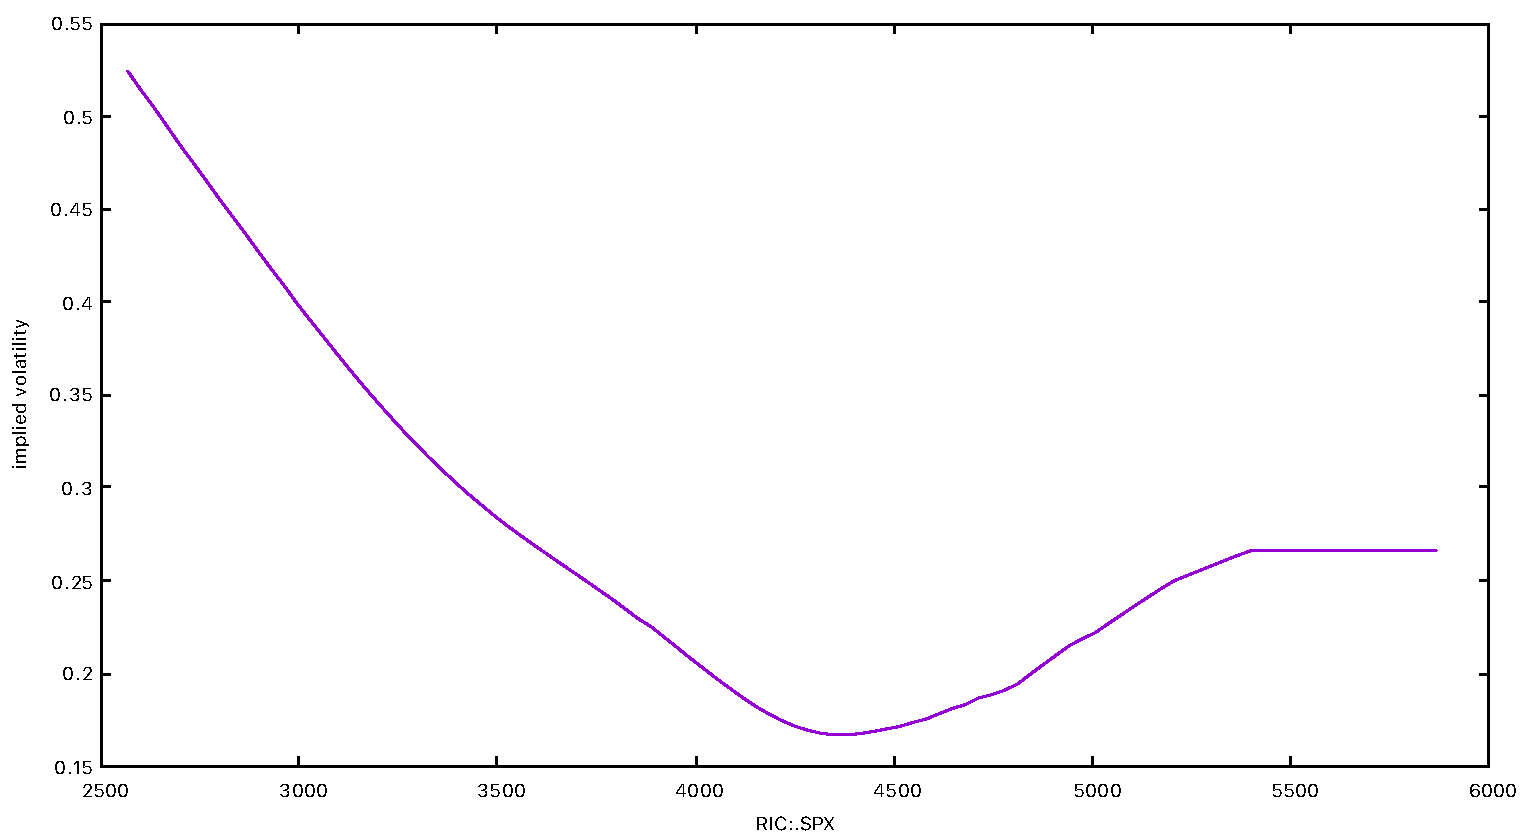
\includegraphics[scale=0.6]{pricing/eq_varianceswap_fig1.pdf}
\end{center}
\caption{Implied volatility of RIC:.SPX at swap maturity $T=0.134247$}
\label{eq_var_swap_fig1}
\end{figure}

\begin{figure}[ht]
\begin{center}
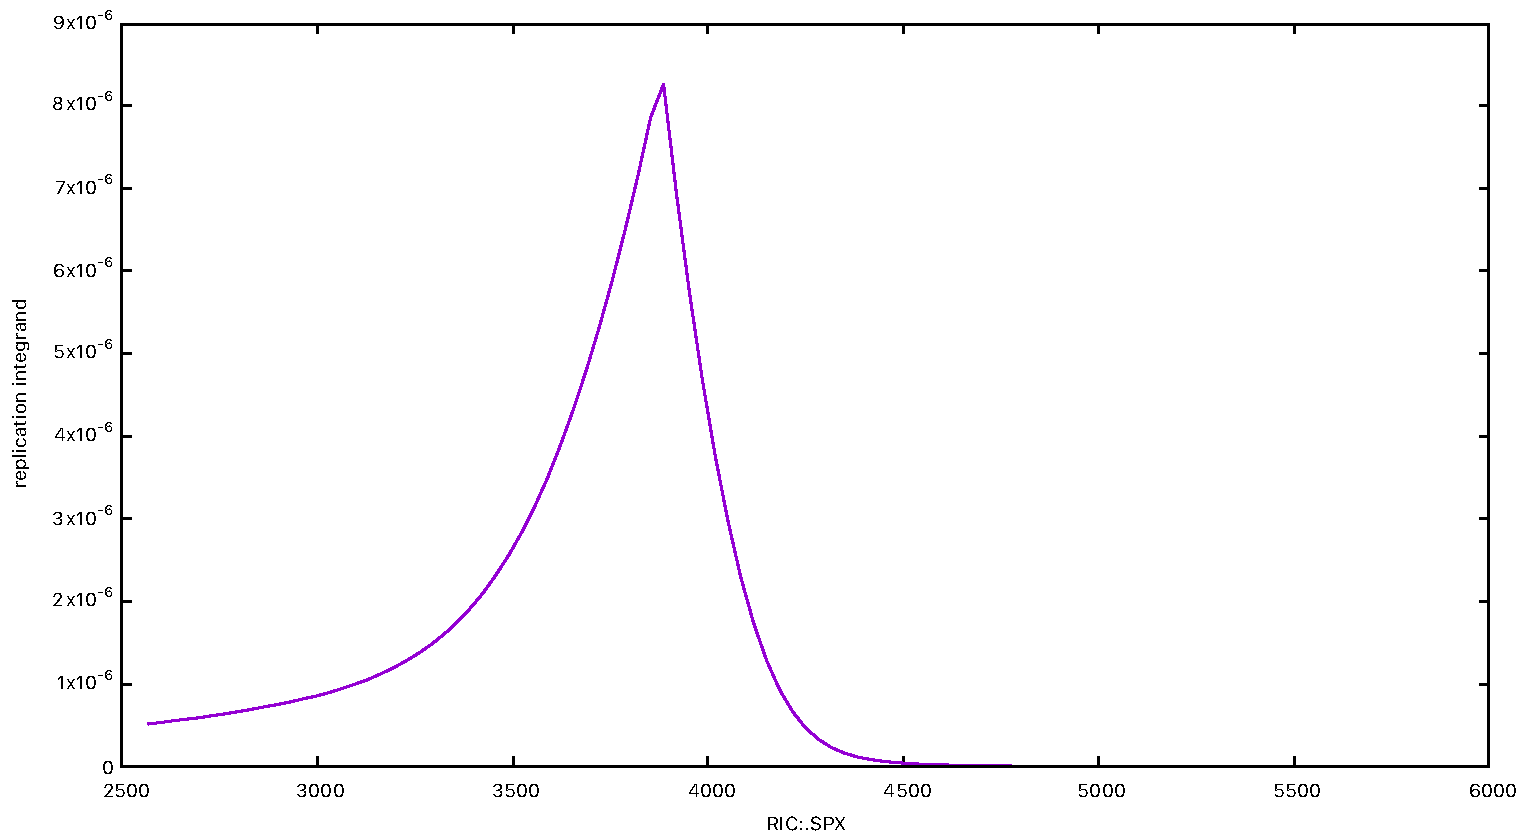
\includegraphics[scale=0.6]{pricing/eq_varianceswap_fig2.pdf}
\end{center}
\caption{The replication integrand, which is given by $\frac{P(K)}{K^2}$ for $K < F$ and $\frac{C(K)}{K^2}$ for $K > F$}
\label{eq_var_swap_fig2}
\end{figure}

\bigskip

\underline{\emph{Total variance:}} The total variance $Var$ in \ref{eq_varianceswap_payoff} is computed as a weighted sum
of the accrued and future variance

$$
Var = \frac{n_1}{n} \text{accrued var} + \frac{n_2}{n} \text{future var}
$$

where

\begin{itemize}
\item $n_1$ is the number of business days between the swap start date and today (both included)
\item $n_2$ is the number of business days between today (excluded) and swap maturity (included)
\item $n$ is the number of business days between the swap start and maturity date (both included)
\end{itemize}

The total variance is available in the additional results under ``totalVariance''. In our case we get

$$
Var = \frac{9}{43}\cdot 0.035178 + \frac{34}{43} 0.062806  = 0.057023
$$

\bigskip

\underline{\emph{Swap NPV:}} The NPV of the swap is finally computed by 

$$
P(0,T) \cdot \omega \cdot N_{var} \cdot 10000 \cdot ( Var - K_{var}  )
$$

with

\begin{itemize}
\item P(0,T) the relevat discount factor for maturity $T$, available in the additional results under ``MaturityDiscountFactor'', in our case $0.993666$
\item the long / short indicator $\omega$ which is $1$ in our case
\item the variance notional $156.25$, available in the additional results under ``VarianceNotional'' (see above for the calculation)
\item the variance strike $0.1024$, available in the additional results under ``VarianceStrike'' (see above for the calculation)
\end{itemize}

This gives a total swap npv of $-70,452.47$ USD.

\bigskip

\underline{\emph{Sensitivity calculation:}} Sensitivities for a variance swap are calculated following a ``bump and
revalue'' approach using the usual configured shift scenarios. The main sensitivities for a variance swap are the
sensitivities to implied volatility (vega) and equity spot price shifts (delta).

There are two major factors impacting the sensitivity to the equity spot:

\begin{itemize}
\item Choice of smile dynamics: ``Sticky Strike'' and ``Sticky Moneyness'' yield different sensitivities to the equity
  spot. The latter choice makes the future variance insensitive to the spot shift, as can be seen from
  \ref{eq_varianceswap_replication}. The former will generate a significant sensitivity to the equity spot on the other
  hand. Both effects are intuitively clear as well.
\item Inlcusion or Exclusion of today's shift contribution (configurable via pricing engine config
  ``StaticTodaysSpot'').
\end{itemize}

Table \ref{eq_var_swap_pricing_sensi_overview} illustrates this by summarizing the sensitivities of our example
trade. Delta is computed w.r.t. a $1\%$ relative shift of the equity spot price, vega w.r.t. to an absolute shift of
$0.01$ in the implied vol and rho w.r.t. a shift of $1$ basispoint on interest rate curves.

\begin{table}[ht]
\begin{center}
\begin{tabular}{l|l|r|r|r}
Smile Dynamics & Todays Shift & Delta & Vega & Rho \\
\hline
Sticky Strike & Included &  -3,622   & 7,357  & -5 \\
Sticky Strike & Excluded &  -4,328   & 7,357  & -5 \\
Sticky Moneyness & Included &  706   & 7,357  & 1 \\
Sticky Moneyness & Excluded &  0 & 7,357  & 1 \\
\end{tabular}
\end{center}
\caption{Variance Swap Sensitivities under different smile dynamics and inclusion / exclusion of today's shift
  contribution}
\label{eq_var_swap_pricing_sensi_overview}
\end{table}
